%%%%%%%%%%%%%%%%%%%% icsc2026_evoking_harmony_4p.tex %%%%%%%%%%%%%%%%%%%%%
% Short (4-page) variant of icsc2026_evoking_harmony.tex

\documentclass[runningheads,a4paper]{llncs}
\usepackage{url}
\usepackage{amsmath}
\usepackage{graphicx}
\usepackage{booktabs}
\usepackage{hyperref}
\hypersetup{hidelinks}
\newcommand{\keywords}[1]{\par\addvspace\baselineskip
\noindent\keywordname\enspace\ignorespaces#1}

\pagestyle{headings}

\begin{document}

\mainmatter

\title{Evoking Harmony via Convolution}
\titlerunning{Evoking Harmony}
\author{AuthorA\inst{1}\and AuthorB\inst{2}}
\authorrunning{AuthorA and AuthorB (or AuthorA et al. if too long)}
\institute{InstituteA \and InstituteB\\ \email{your.email@yourdomain.com}}

\maketitle

\begin{abstract}
I demonstrate how to impart, or evoke, the tonality of a chord from a source 
sound while, at the same time, minimizing artifacts and creating an 
interesting effect. Conceptually, the effect consists of convolving the 
source signal with the pitch-classes of the chord. I develop alternative 
implementations of this effect in Csound, analyze the characteristics of each 
implementation, and demonstrate some musical uses.
\keywords{csound harmony convolution}
\end{abstract}

\section{Introduction}

When I was a boy my father drove with me several times from our home in Salt 
Lake City to Los Angeles on business trips. He drove across the desert without 
stopping. Long stretches of the highway were empty and straight. I lay with my 
head against the window post and listened to the sound of the car, the road, 
and the wind. In the rushing noise I heard whistling voices singing 
counterpoint.

Ever since that time I have wondered if there is some way to produce this 
effect in electroacoustic music. I have now performed some experiments using 
Csound \cite{csound_home}, and here I report my results. These include some 
user-defined opcodes, a Csound test orchestra, some input soundfiles, the 
resulting test soundfile, and an example piece demonstrating some musical 
uses. All of these materials are available at my Github respository 
\cite{gogins_github_io}.

In brief, it is possible to approximate what I heard by convolving a source 
signal with the pitch-classes of a chord. This functions as a filter to 
emphasize those frequencies of the source that also occur in the chord. I call 
this effect \emph{chord convolution}.

\emph{To convolve with the pitch-classes of a chord} means to convolve with an 
impulse response consisting of all sinusoids within the range of human 
hearing that belong to any of the pitch-classes of the chord. For example, the 
chord C major consists of pitch-classes C, E, and G. For the pitch-class C, 
there is one sinusoid at 32.703 Hz, one at 65.406 Hz, and so on up to 
16,744.036 Hz; for G, one sinusoid at 41.203 Hz and so on up to 21,906.164 Hz; 
and for E, one at 48.999 Hz and so on up to 12,543.854 Hz. Please note, 
pitch-classes are not limited to 12-tone equal temperament; \emph{pitch-class} 
is simply an equivalence class that identifies frequencies \emph{modulo} the 
octave. 

The main artifact of concern in this case is the smearing caused by 
convolution. Because in all representations of sound there is an irreducible 
Gabor uncertainty of information, a smallest possible area of time $\times$ 
frequency which implies an indeterminacy relation between time and frequency 
\cite{gabor1946theory}, this artifact cannot be eliminated, but it can be 
minimized. We hear it as ringing (smearing of time) or blurring of pitch 
(smearing of frequency). The chord impulse response can be made shorter to 
increase time resolution at the cost of frequency resolution, or it can be made 
longer to increase frequency resolution at the cost of time resolution. The 
shortest possible impulse response consists of one cycle of the fundamental 
frequency of the chord. The best value of this tradeoff may be different for 
different source signals and for different musical purposes, so it is made into 
a parameter for the effect --- the duration of the chord impulse response.

Human factors impose other fundamental limitations. People cannot identify 
pitch within much less than 50 milliseconds, and features of interest in the 
source signal, if not sparser than the convolution ring, will be smeared 
together at the chord frequencies, which may or may not be desirable.

A further optimization consists of convolving with a separate impulse response 
for each component sinusoid of the chord's pitch-classes, making the impulse 
shorter as the frequency increases. This is a form of multi-resolution signal 
processing. As a result, the smearing is larger at lower frequencies and 
smaller at higher freqencies. This not only significantly reduces the ringing 
artifact, but also increases the subjective time resolution of the effect.

\section{Methods}

Direct convolution with $N$ cycles of each chord partial is optimal but
impractical; I did not implement it. Three efficient variants are compared
(Table~\ref{tab:udos}). All accept up to six chord voices (MIDI key numbers,
possibly fractional), wet/dry mix, and output gain; full signatures are in the
repository \cite{gogins_github_io}.

\begin{table}[t]
\centering
\caption{Chord-convolution UDOs in Csound.}
\label{tab:udos}
\begin{tabular}{@{}lll@{}}
\toprule
UDO & Basis & Main control \\
\midrule
\texttt{ImpartChordWithFilterbank} & \texttt{resonz} \cite{csoundmanualresonz}
  & bandwidth (cents) \\
\texttt{ImpartChordWithFtconv} & \texttt{ftconv} \cite{csoundmanualftconv}
  & impulse width (cycles) \\
\texttt{ImpartChordWithMultiFtconv} & per-partial \texttt{ftconv}
  & width (cycles per partial) \\
\bottomrule
\end{tabular}
\end{table}

The filter bank uses one IIR bandpass per partial; narrow bandwidth increases
frequency resolution and ringing. Partitioned convolution uses a single
finite impulse response per partial. Multi-\texttt{ftconv} applies a separate
partitioned convolution at each partial, combining multi-resolution smearing
with reasonable CPU cost.

\section{Results}

Four source signals probe the implementations: (1)~unit impulse;
(2)~rain (noisy, unpitched); (3)~struck steel bowl (pitched, inharmonic);
(4)~rainspout with radio (mixed time scales). Each was processed with six
settings: filter bank at 100 and 5 cents; partitioned convolution at one
fundamental cycle; multi-resolution convolution at 8 and 32 cycles per
partial. A test soundfile cycles through all combinations; a separate piece
applies the effect to field recordings.

Figure~\ref{fig:smearing} summarizes impulse responses (narrow spectrogram
window). Single-resolution \texttt{ftconv} beats the filter bank on time
resolution; multi-\texttt{ftconv} is sharpest at high frequencies. Wider
settings (5 cents, 32 cycles) lengthen ringing, as expected.

\begin{figure}[t]
 \centering
 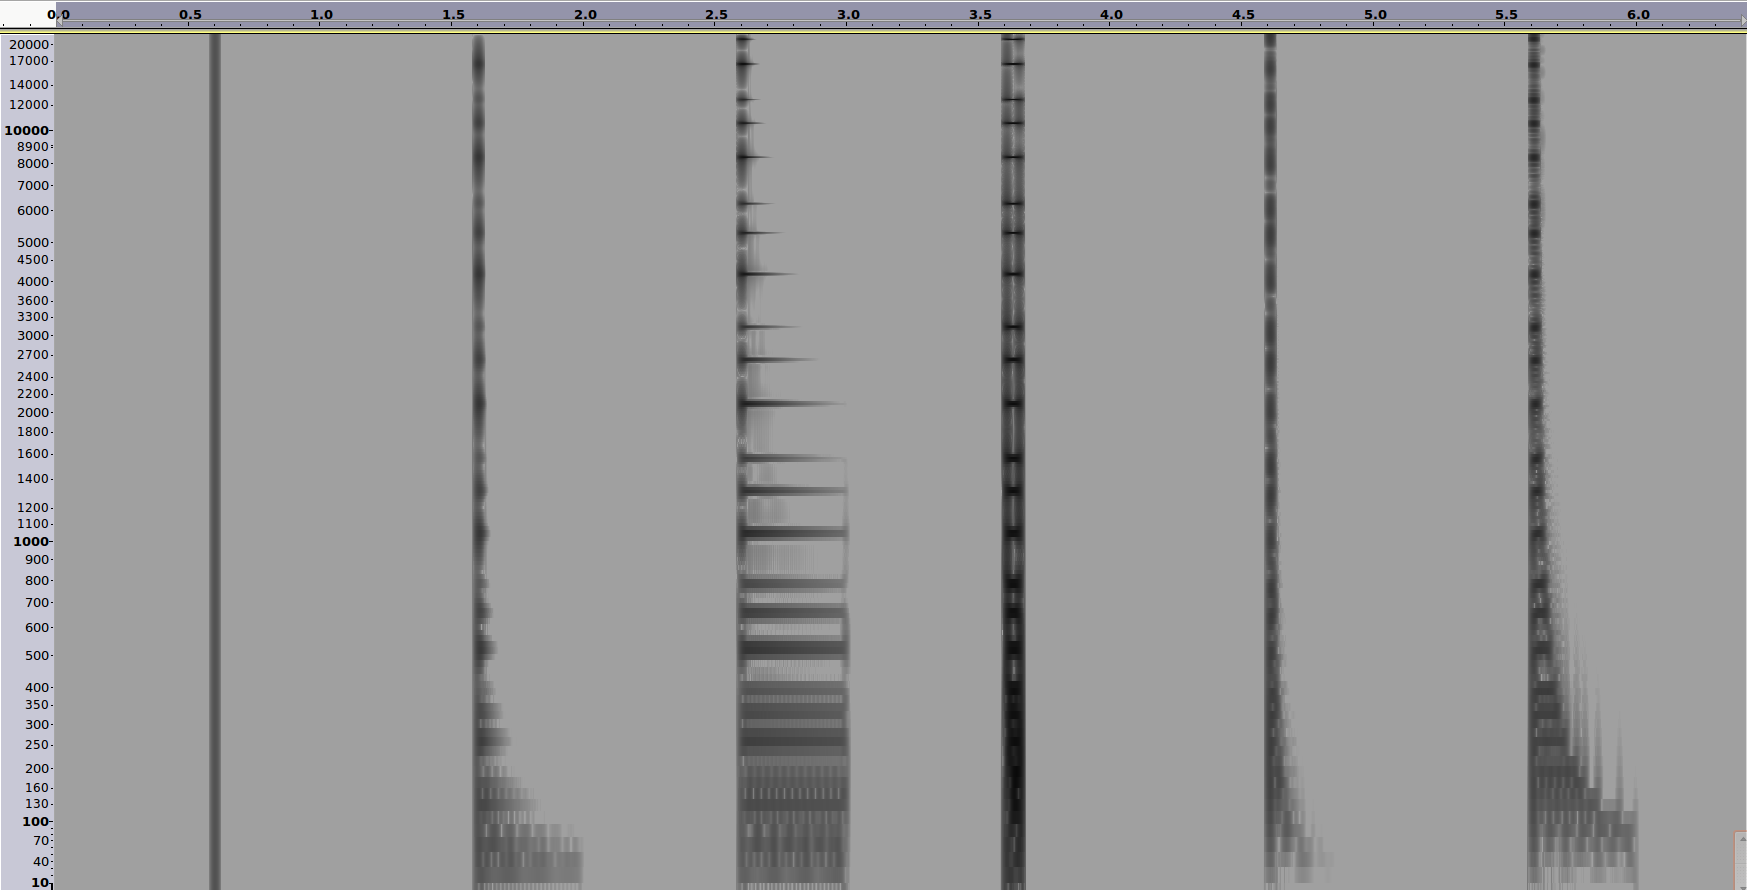
\includegraphics[width=\linewidth,keepaspectratio=true]{smearing.png}
 \caption{Impulse responses (narrow analysis window). Columns: unprocessed;
 filter bank 100 cents; 5 cents; \texttt{ftconv} (1 cycle); multi-\texttt{ftconv}
 8 cycles; 32 cycles.}
 \label{fig:smearing}
\end{figure}

Figure~\ref{fig:rain} shows rain (representative unpitched source; bowl and
rainspout behave similarly---harmonic shadow on pitched sources, arpeggiated
``dancing'' with a wet filter bank on sparse material). Narrow filter bands do
not always sound \emph{more} tonal: on rain, 100 cents sounds stronger than
5 cents because resonances overlap; on the bowl, narrow bands often fail to
catch inharmonic partials. Multi-\texttt{ftconv} at 8 cycles balances soft
tonality with sharper attacks than plain \texttt{ftconv}. See 
\cite{evoking_harmony_test} for more results.

\begin{figure}[t]
 \centering
 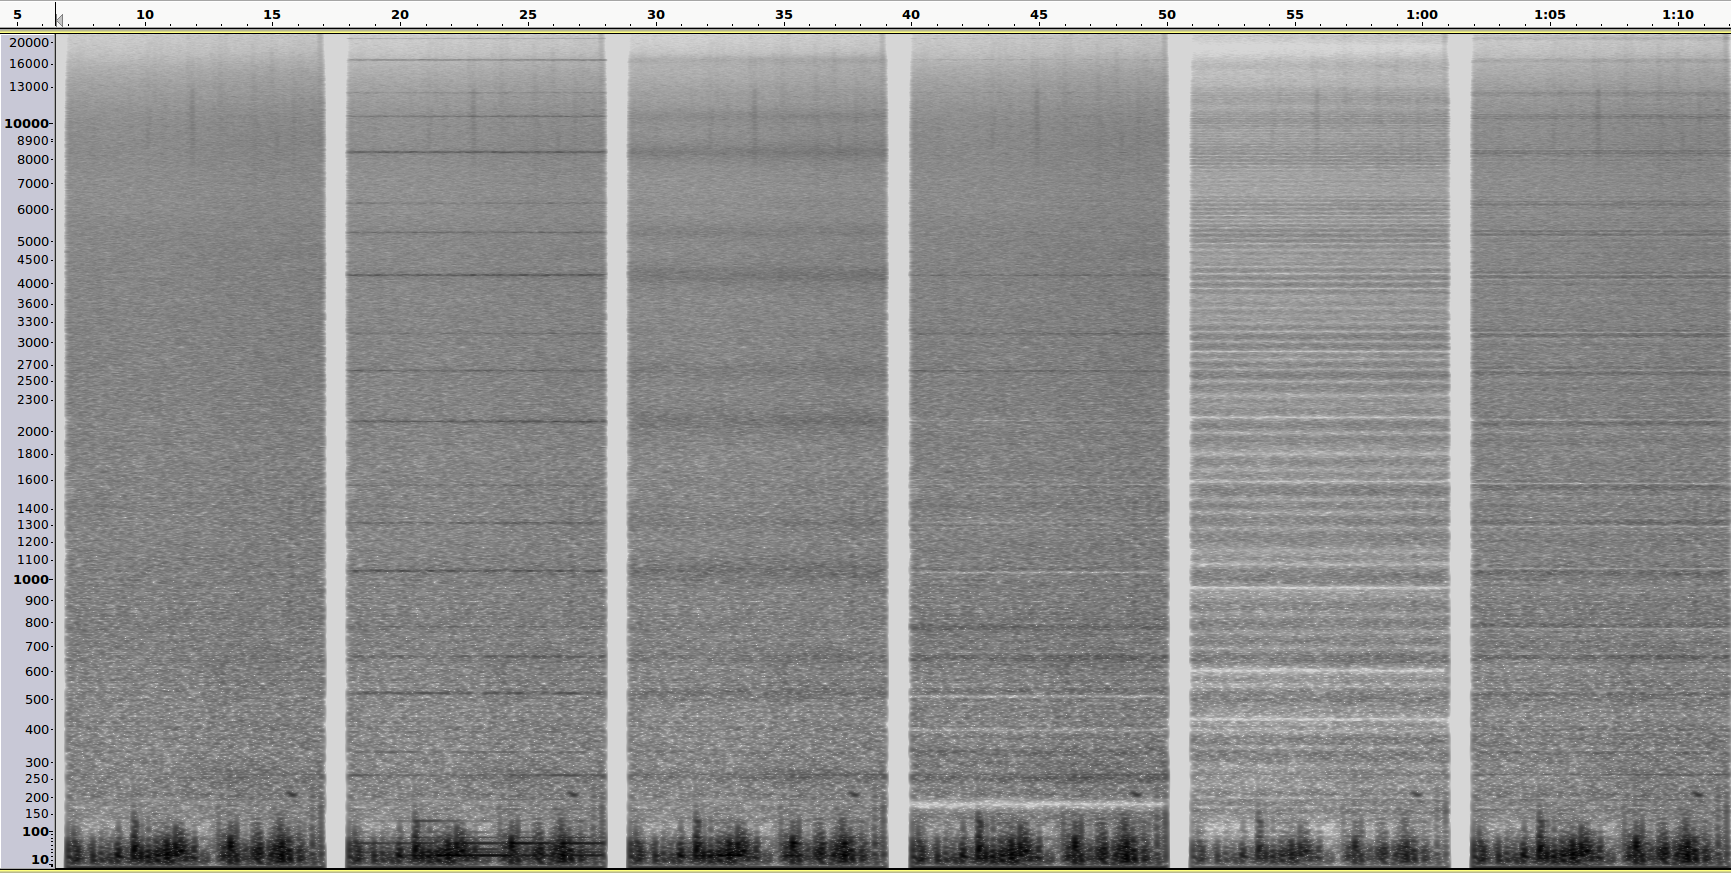
\includegraphics[width=\linewidth,keepaspectratio=true]{rain.png}
 \caption{Rain: same six processing settings as Fig.~\ref{fig:smearing}.}
 \label{fig:rain}
\end{figure}

A sound walk with a field recorder at twilight alongside a ruined castle in a 
French village demonstrates various applications of harmonic evocation to 
ambient sounds \cite{evoking_harmony_sound_walk}

\section{Discussion}

Chord convolution resembles comb filtering or a channel vocoder, but chord
tonality is audible when time/frequency settings match the source. It works
best when harmonic sensation is subtle---on unpitched or varied textures, or as
a ``harmonic shadow'' on pitched sources in a different key. A wetter, longer
smear (filter bank) can suggest ringing arpeggios on rhythmic material.
Implementation and parameter choices are audible but nuanced; supplementary
figures and audio on GitHub cover bowl, rainspout, and time-domain responses.

\paragraph{Note.}
This abbreviated version was edited for length with assistance from generative
AI tools; the author reviewed the text and retains responsibility for all
technical content.

\bibliographystyle{unsrt}
\bibliography{icsc2026_evoking_harmony}

\end{document}
